\subsection{Optimierung}

Im Anschluss an die Synthese wird das Stubfilter optimiert. Dabei werden die Schranken des Optimieres so gesetzt, dass sich der Sperrbereich verbessert, während der Equirippel im Passband gleich bleiben soll. In Abb. \ref{fig:vor-nach-optimierung} wird das synthetisierte Stubfilter (rot,blau) dem optimierten Stubfilter (braun, magenta) gegenübergestellt. 

Ein Vergleich des Passbands zeigt, dass sich die Filterordung nach der Optimierung von 5 auf 9 erhöht hat. Dies leuchtet nicht sofort ein, weil das Stubfilter vor und nach der Optimierung immer noch aus gleich vielen Elementen besteht. Der Grund für die Erhöhung der Filterordnung ist, dass sich beim Einfügen der Unit-Elementen vier zusätzliche Pol- und Nullstellen eingeschlichen haben. Die Unit-Elemte sind aber so berechnet, dass sich die zusätzlichen Pol- und Nullstellen allesamt aufheben. Aus diesem Grund sieht der Frequenzgang nach der Kuroda Transformation immer noch genau gleich wie nach der Richard's Frequenztransformation aus. Nach der Synthese beinhaltet das synthetisierte Stubfilter also vier redundante Elemente die gar keinen Einfluss auf den Frequenzgang haben. 

Wird das Stubfilter optimiert so verschieben sich die vier Pol- und Nullstellen und sie werden im Passband ersichtlich, wobei sich gleichzeitig die Filterordnung erhöht


\begin{figure}[h!]
    \centering
    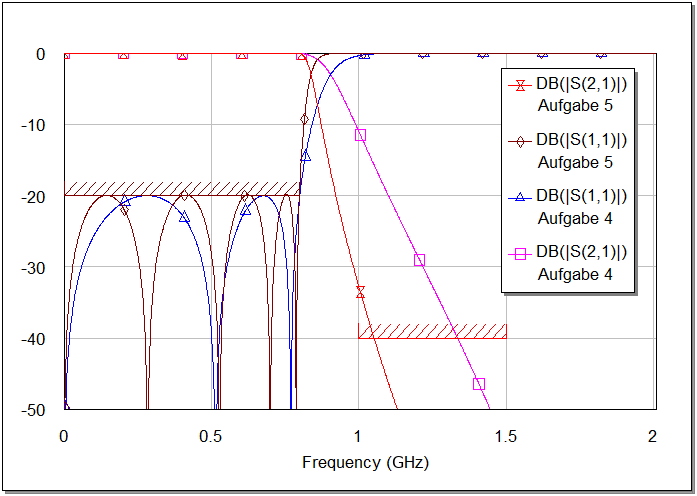
\includegraphics[width=\linewidth]{images/graph-optimierung}
    \caption{Stubfilter vor und nach Optimierung, von Frau Spuhler zur Verfügung gestellt}
    \label{fig:vor-nach-optimierung}
\end{figure}

